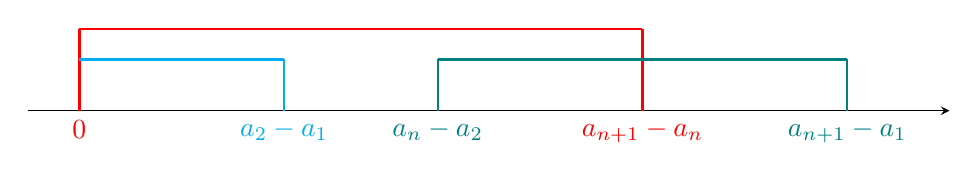
\begin{tikzpicture}[>=stealth, scale=1.3]
        % 数轴
        \draw[->] (-0.5,0) -- (8.5,0);
        
        % 坐标点定义 (根据相对位置设定坐标)
        \coordinate (O) at (0,0);
        \coordinate (A) at (2,0);   % a2 - a1
        \coordinate (B) at (3.5,0); % an - a2
        \coordinate (C) at (5.5,0); % an+1 - an
        \coordinate (D) at (7.5,0); % an+1 - a1
        
        % 刻度标签 (颜色参考原图手写笔记)
        \node[below, red] at (O) {$0$};
        \node[below, cyan] at (A) {$a_2-a_1$};
        \node[below, teal] at (B) {$a_n-a_2$};
        \node[below, red] at (C) {$a_{n+1}-a_n$};
        \node[below, teal] at (D) {$a_{n+1}-a_1$};
        
        % 区间绘制
        % 红色区间 [0, an+1 - an]
        \draw[red, thick] (0, 0.8) -- (5.5, 0.8);
        \draw[red, thick] (0, 0) -- (0, 0.8);
        \draw[red, thick] (5.5, 0) -- (5.5, 0.8);
        
        % 绿色区间 [an - a2, an+1 - a1]
        \draw[teal, thick] (3.5, 0.5) -- (7.5, 0.5);
        \draw[teal, thick] (3.5, 0) -- (3.5, 0.5);
        \draw[teal, thick] (7.5, 0) -- (7.5, 0.5);
        
        % 蓝色区间 [0, a2 - a1] (包含在红色区间内)
        \draw[cyan, thick] (0, 0.5) -- (2, 0.5);
        \draw[cyan, thick] (2, 0) -- (2, 0.5);
        
    \end{tikzpicture}